%%%%%%%%%%%%%%%%%%%%%%%%%%%%%%%%%%%%%%%%%%%%%%%%%%%%%%%%%%%%%%%%%%%%%%%%%%%%%%%%%%%%%%%%%%%%%%%%%%%%%%%%%%%%%%%%%%%%%%%%%%%%%%%%%%%%%%%%%%%%%%%%%%%%%%%%%%%
% This is just an example/guide for you to refer to when submitting manuscripts to Frontiers, it is not mandatory to use Frontiers .cls files nor frontiers.tex  %
% This will only generate the Manuscript, the final article will be typeset by Frontiers after acceptance.   
%                                              %
%                                                                                                                                                         %
% When submitting your files, remember to upload this *tex file, the pdf generated with it, the *bib file (if bibliography is not within the *tex) and all the figures.
%%%%%%%%%%%%%%%%%%%%%%%%%%%%%%%%%%%%%%%%%%%%%%%%%%%%%%%%%%%%%%%%%%%%%%%%%%%%%%%%%%%%%%%%%%%%%%%%%%%%%%%%%%%%%%%%%%%%%%%%%%%%%%%%%%%%%%%%%%%%%%%%%%%%%%%%%%%

%%% Version 3.4 Generated 2022/06/14 %%%
%%% You will need to have the following packages installed: datetime, fmtcount, etoolbox, fcprefix, which are normally inlcuded in WinEdt. %%%
%%% In http://www.ctan.org/ you can find the packages and how to install them, if necessary. %%%
%%%  NB logo1.jpg is required in the path in order to correctly compile front page header %%%

\documentclass[utf8]{FrontiersinHarvard}

%\setcitestyle{square} % for Physics and Applied Mathematics and Statistics articles
\usepackage{url,hyperref,lineno,microtype,subcaption}
\usepackage[onehalfspacing]{setspace}

\linenumbers


% BELOW TAKEN FROM rticles plos template
%
% amsmath package, useful for mathematical formulas
\usepackage{amsmath}
% amssymb package, useful for mathematical symbols
\usepackage{amssymb}

% hyperref package, useful for hyperlinks
\usepackage{hyperref}

% graphicx package, useful for including eps and pdf graphics
% include graphics with the command \includegraphics
\usepackage{graphicx}

% Sweave(-like)
\usepackage{fancyvrb}
\DefineVerbatimEnvironment{Sinput}{Verbatim}{fontshape=sl}
\DefineVerbatimEnvironment{Soutput}{Verbatim}{}
\DefineVerbatimEnvironment{Scode}{Verbatim}{fontshape=sl}
\newenvironment{Schunk}{}{}
\DefineVerbatimEnvironment{Code}{Verbatim}{}
\DefineVerbatimEnvironment{CodeInput}{Verbatim}{fontshape=sl}
\DefineVerbatimEnvironment{CodeOutput}{Verbatim}{}
\newenvironment{CodeChunk}{}{}

% cite package, to clean up citations in the main text. Do not remove.
\usepackage{cite}

\usepackage{color}

% Below is from frontiers

% Leave a blank line between paragraphs instead of using \\


\def\keyFont{\fontsize{8}{11}\helveticabold }


%% ** EDIT HERE **
%% PLEASE INCLUDE ALL MACROS BELOW

%% END MACROS SECTION


% tightlist command for lists without linebreak
\providecommand{\tightlist}{%
  \setlength{\itemsep}{0pt}\setlength{\parskip}{0pt}}




\def\Authors{
  Giulia Terlecki\,\textsuperscript{1*},
  Silvina Botta\,\textsuperscript{2},
  Luis Gustavo Cardoso\,\textsuperscript{1}}

\def\Address{

  \textsuperscript{1} Laboratório de Dinâmica Populacional Pesqueira,
Instituto de Oceanografia, Programa de pós-graduação em Oceanografia
Biológica, Universidade Federal do Rio Grande,  Rio Grande,  Rio Grande
do Sul,  Brazil
  
  \textsuperscript{2} Department X, Universidade Federal do Rio
Grande,  Rio Grande,  Rio Grande do Sul,  Brazil
  }

  \def\corrAuthor{Giulia
Terlecki}\def\corrAddress{,  }\def\corrEmail{\href{mailto:giuliaterlecki@gmail.com}{\nolinkurl{giuliaterlecki@gmail.com}}}
  \def\firstAuthorLast{Terlecki {et~al.}}
  
  
  
  


\begin{document}

\onecolumn
\firstpage{1}


\title[Habitat de Tubarões no Atlântico Sul]{Uso de Habitat de Tubarões
Azul e Anequim no Oceano Atlântico Sul}
\author[\firstAuthorLast]{\Authors}
\address{} %This field will be automatically populated
\correspondance{} %This field will be automatically populated

\extraAuth{}% If there are more than 1 corresponding author, comment this line and uncomment the next one.
%\extraAuth{corresponding Author2 \\ Laboratory X2, Institute X2, Department X2, Organization X2, Street X2, City X2 , State XX2 (only USA, Canada and Australia), Zip Code2, X2 Country X2, email2@uni2.edu}


\maketitle

\begin{abstract}
Abstract length and content varies depending on article type. Refer to
\url{http://www.frontiersin.org/about/AuthorGuidelines} for abstract
requirement and length according to article type.

\tiny
 \keyFont{ \section{Keywords:} tubarao azul, estoques
pesqueiros, microquimica, isotopos, uso de
habitat} %All article types: you may provide up to 8 keywords; at least 5 are mandatory.
\end{abstract}

\section*{Introduction}\label{introduction}
\addcontentsline{toc}{section}{Introduction}

O tubarão azul (\emph{Prionace glauca}) e o anequim (\emph{Isurus
oxyrinchus}) são duas das principais espécies de tubarões pelágicos do
Atlântico, com distribuições amplas e migratórias que as tornam
vulneráveis à exploração pesqueira \citep{Campana2004, Stevens2010}.
Essas espécies desempenham papéis ecológicos fundamentais nos
ecossistemas marinhos, regulando as populações de suas presas e
contribuindo para a manutenção do equilíbrio ecológico
\citep{Heithaus2008}. Estudos recentes destacam a importância de
compreender a conectividade populacional desses tubarões para
desenvolver estratégias de manejo que considerem sua natureza
transoceânica e evitem o declínio populacional
\citep{Queiroz2019, Ferreira2017}.

O uso de análises isotópicas e microquímicas em vértebras de tubarões
tem se mostrado uma ferramenta valiosa para rastrear padrões de
migração, conectividade e mudanças ontogenéticas em hábitos alimentares
\citep{Estrada2006, Hussey2015}. Através dessas análises, é possível
identificar as áreas de alimentação e os movimentos sazonais das
espécies, fornecendo insights sobre as dinâmicas de habitat e as
interações tróficas ao longo de diferentes fases da vida dos tubarões
\citep{Carlisle2015, MacNeil2005}.

\begin{figure}
\centering
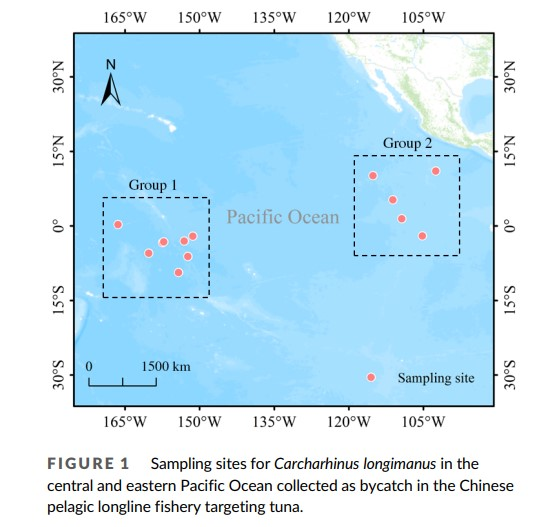
\includegraphics[width=0.5\textwidth,height=\textheight]{stockarea.jpg}
\caption{Dois locais analisados no estudo}
\end{figure}

\subsubsection*{Fórmula para Posição
Trófica}\label{fuxf3rmula-para-posiuxe7uxe3o-truxf3fica}
\addcontentsline{toc}{subsubsection}{Fórmula para Posição Trófica}

Para estimar a posição trófica dos tubarões analisados, foi utilizada a
seguinte fórmula de enriquecimento isotópico de nitrogênio entre
predador e presa:

\[
\Delta^{15}N = \delta^{15}N_{predador} - \delta^{15}N_{presa}
\]

onde \(\delta^{15}N\) representa o valor isotópico de nitrogênio nas
amostras de vértebras, possibilitando inferir a posição trófica e os
hábitos alimentares ontogenéticos dos indivíduos
\citep{Shiffman2019, Rooker2008}.

Estudos como o de \citet{Queiroz2019} demonstram que o tubarão azul
exibe conectividade entre regiões do Atlântico, reforçando a necessidade
de uma abordagem de manejo cooperativa entre diferentes países. Este
estudo visa investigar a sobreposição de nicho entre o tubarão azul e o
anequim no Atlântico Sul e avaliar a conectividade do tubarão azul entre
as regiões sudoeste e sudeste do oceano.

Results \{-\}

Espera-se que os resultados deste estudo revelem uma sobreposição
significativa de nicho entre o tubarão azul (\emph{Prionace glauca}) e o
anequim (\emph{Isurus oxyrinchus}) no Atlântico Sul. A análise isotópica
deverá indicar variações na posição trófica entre as fases ontogenéticas
dos tubarões, evidenciando especializações alimentares em diferentes
estágios de vida \citep{Carlisle2015, Estrada2006}.

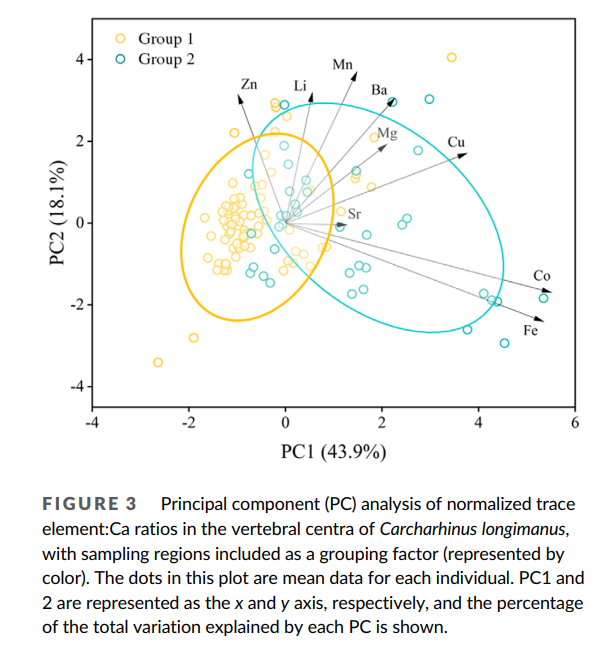
\includegraphics[width=0.5\textwidth,height=\textheight]{grupo2.png}
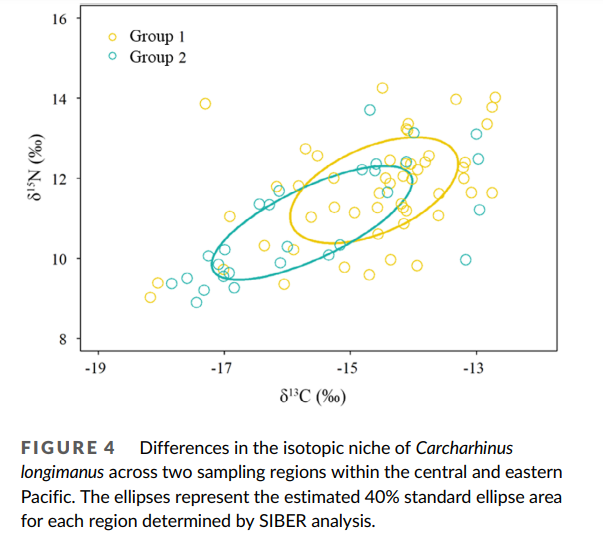
\includegraphics[width=0.5\textwidth,height=\textheight]{group22.png}

(mapa do Atlântico Sul) com as rotas de migração estimadas dos tubarões
azul e anequim, destacando os pontos de coleta das amostras de
vértebras, é uma adição importante. Esse mapa visualizaria as conexões
entre as regiões sudoeste e sudeste do Atlântico e outras áreas
relevantes, demonstrando visualmente a distribuição e possíveis rotas
migratórias das duas espécies.

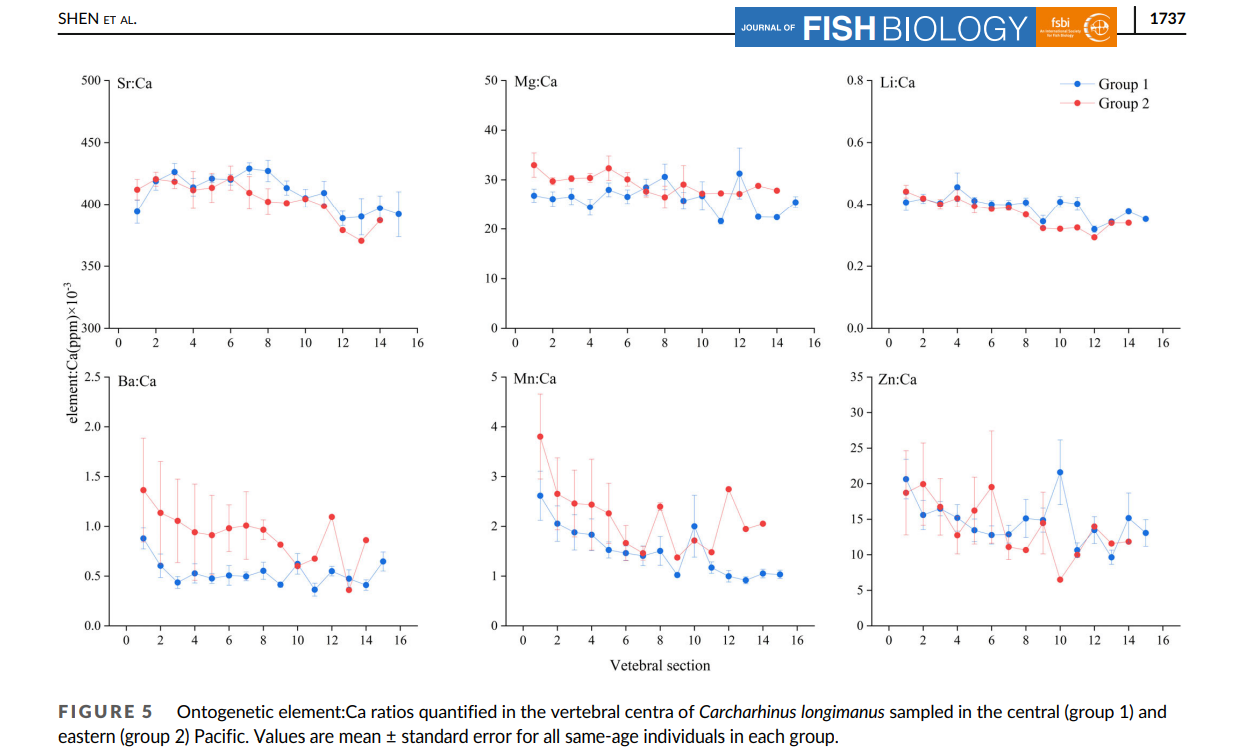
\includegraphics[width=0.5\textwidth,height=\textheight]{group23.png} \#
Discussion

Os resultados sugerem uma significativa sobreposição de nicho entre o
tubarão azul (Prionace glauca) e o anequim (Isurus oxyrinchus) no
Atlântico Sul, com ambos ocupando habitats pelágicos similares para
alimentação e reprodução. Essa sobreposição de nicho pode indicar
competição por recursos nas áreas onde as duas espécies coabitam, o que
pode ter implicações importantes para a gestão pesqueira, especialmente
considerando que ambas as espécies já são vulneráveis à exploração.

As análises isotópicas revelaram variações na posição trófica ao longo
das diferentes fases ontogenéticas dos tubarões, sugerindo que essas
espécies adaptam suas dietas conforme amadurecem. Esse comportamento
pode indicar uma especialização alimentar que permite às espécies
explorar diferentes recursos tróficos, minimizando a competição em
determinadas fases de vida. Além disso, a conectividade transoceânica
observada nas amostras de tubarão azul reforça a importância de
estratégias de manejo colaborativas entre as nações do Atlântico, visto
que essas populações podem depender de áreas de alimentação e reprodução
em várias regiões geográficas.

Essas descobertas oferecem uma base valiosa para futuras recomendações
de conservação, que devem considerar a dinâmica de conectividade e a
especialização trófica ao longo da vida dessas espécies.

\section*{Disclosure/Conflict-of-Interest
Statement}\label{disclosureconflict-of-interest-statement}
\addcontentsline{toc}{section}{Disclosure/Conflict-of-Interest
Statement}

The authors declare that the research was conducted in the absence of
any commercial or financial relationships that could be construed as a
potential conflict of interest.

\section*{Author Contributions}\label{author-contributions}
\addcontentsline{toc}{section}{Author Contributions}

Giulia Terlecki: Led study design, objectives, and methodology.
Conducted isotopic and microchemical analyses, interpreted data, and
drafted the manuscript. Approved the final version and is accountable
for data accuracy and conclusions.

Silvina Bota: Provided technical support in microchemical methodology
and contributed to the critical review, ensuring methodological
accuracy. Approved the final version and is responsible for the
precision of microchemical analyses.

Luis Gustavo Cardoso: Offered guidance on study conception, statistical
analysis, and manuscript revisions, contextualizing findings within the
literature. Approved the final version and ensures content integrity.

\section*{Acknowledgments}\label{acknowledgments}
\addcontentsline{toc}{section}{Acknowledgments}

This study was supported by funding from the Coordination for the
Improvement of Higher Education Personnel (CAPES), the National Council
for Scientific and Technological Development (CNPq), and the Office of
the Dean of Extension and Culture (PROEX). We also thank the Institute
of Coastal and Marine Ecosystem Research (ICACAT) for additional
support.



\end{document}
